\chapter{Analog amplifiers}
One of the goals of the thesis is to automate the design of analog amplifiers. These are electronic circuits that are used to increase the input signal with the minimum amount of distortion to the output signal. There are two amplifiers used in this thesis which are discussed below.

\section{Single stage common emitter amplifier} \label{ce-amp}
The single stage common emitter amplifier was chosen because it belongs to the most commonly used examples of analog amplifiers in class A. The circuit diagram is shown in figure \ref{ce-amplifier}. We can find a thorough description of this circuit in \cite{the-art-of-electronics}.

\begin{figure}[H]
    \centering
    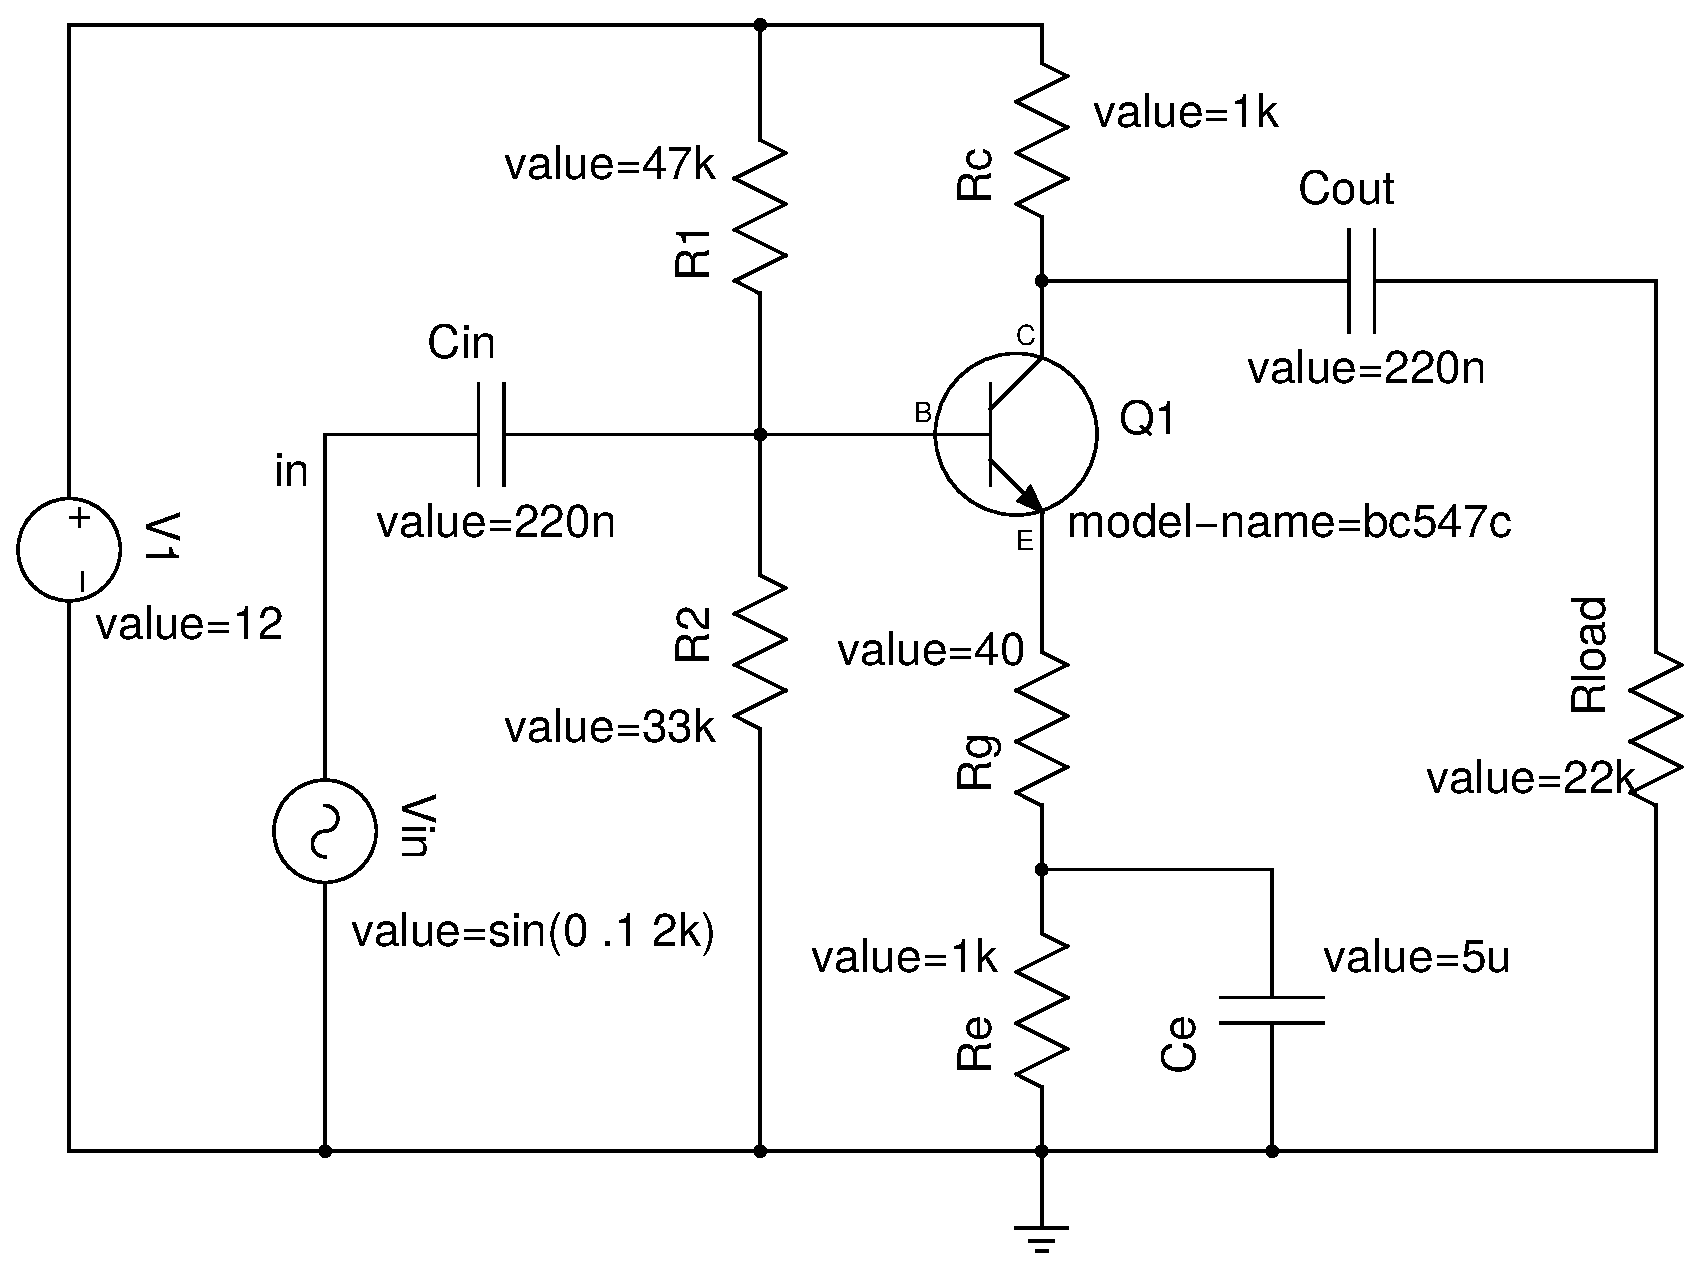
\includegraphics[scale=0.35]{ce-amplifier}
    \label{ce-amplifier}
    \caption{Circuit diagram for the common emitter amplifier}
\end{figure}

Resistors $R1$ and $R2$ are used to bias transistor $Q1$ in order to set the quiescent point of the transistor to the middle of its DC load line so that the collector of $Q1$ is put at $1/2$ of the supply voltage $V1$. This allows the maximum symmetrical swings of the output signal without clipping (flattening of the top or the bottom of the waveform). The collector voltage depends on the collector current (quiescent current), equation \ref{collector-voltage}. This current depends on the applied base bias and the values of $Rc$ and $Re$.

\begin{equation} \label{collector-voltage}
    V_c = V1 - I_c \cdot Rc
\end{equation}

Instead of using a voltage divider for biasing, it is possible to use only resistor $R1$, but this approach would make the quiescent point highly dependent on the current gain $\beta$ of the transistor. This parameter varies considerably in every transistor and the manufacturer usually specifies only a certain range of $\beta$. For this reason, we use a voltage divider constituted by $R1$ and $R2$ which impedance should be small compared with the impedance looking into the transistor base, formula \ref{divider-impedance}. This will give us a divider which is stiff enough so that the quiescent point is insensitive to variations in transistor $\beta$. However, the current flowing in the divider should not be unnecessarily large as it affects the overall consumption of the amplifier.

\begin{equation} \label{divider-impedance}
    R1 \| R2 \ll \beta Re
\end{equation}

Capacitors $Cin$ and $Cout$ form high pass filters and they are used as coupling capacitors to separate the AC signals from the DC voltage used to set up the amplifier. Their values are chosen so that the capacitors have low impedance for the desired input and output signal frequencies. This ensures that the signal's average is zero, as the capacitors pass only AC signals and block any DC component.

The input voltage $Vin$ causes a wiggle in the base voltage. The emitter voltage follows the base voltage which causes a wiggle in the emitter and also collector current. The output voltage which is the collector voltage depends on the current flowing through $Rc$, equation \ref{collector-voltage}. When this current rises, the collector voltage drops and vice versa. That means that the amplifier also inverts the input signal, figure \ref{ce-amplifier-sim}. The output AC signal is then superimposed on the collector DC voltage and the DC component is subsequently filtered out by the capacitor $Cout$ (high pass filter).

Capacitor $Ce$ is used to reach the amplifier's maximum gain. The values of $Re$ and $Rg$ set the emitter voltage which affects the amplifier's gain and we usually want these values to be as low as possible since this gives us the highest gain. However, if the emitter voltage is too low, it will vary significantly as the base-emitter drop varies with temperature. The solution is to bypass the $Re$ resistor so that the impedance for the emitter will vary according to the signal's frequency. The bypass capacitor $Ce$ is an open circuit component for DC bias and the emitter voltage depends on both $Re$ and $Rg$ which allows stable biasing. For higher frequency signals, the bypass capacitor short circuits $Re$ and the emitter voltage now depends mostly on $Re$ which value sets the maximum gain.

The analytical calculation for this circuit is beyond the scope of this thesis and it is left up to the evolutionary algorithms. The subject of the optimization are elements $R1$, $R2$, $Re$, $Rg$, $Rc$, $Cin$, $Ce$ and $Cout$. These elements represent the solution variables in the evolution strategies and make up the vector $\vec{x}$ which is thoroughly discussed in section \ref{mutation-section}. In this case, we optimize 8 components in the circuit so the search space has 8 dimensions.

\section{Two stage amplifier}
We can see the circuit diagram for a two stage amplifier on figure \ref{ce-amplifier-2stage}. The functionality and structure of the circuit are similar to the previous one with the difference that now we use two transistors connected in a cascade where transistor $Q1$ sends its output to the base of transistor $Q2$. This circuit was chosen as a more difficult problem to optimize, since the structure is twice as complicated as in the previous amplifier. The subject of the optimization are all the resistors and capacitors in the diagram apart from resistor $Rload$, so we have 14 compontents to optimize which makes the search space 14-dimensional.

\begin{figure}[H]
    \centering
    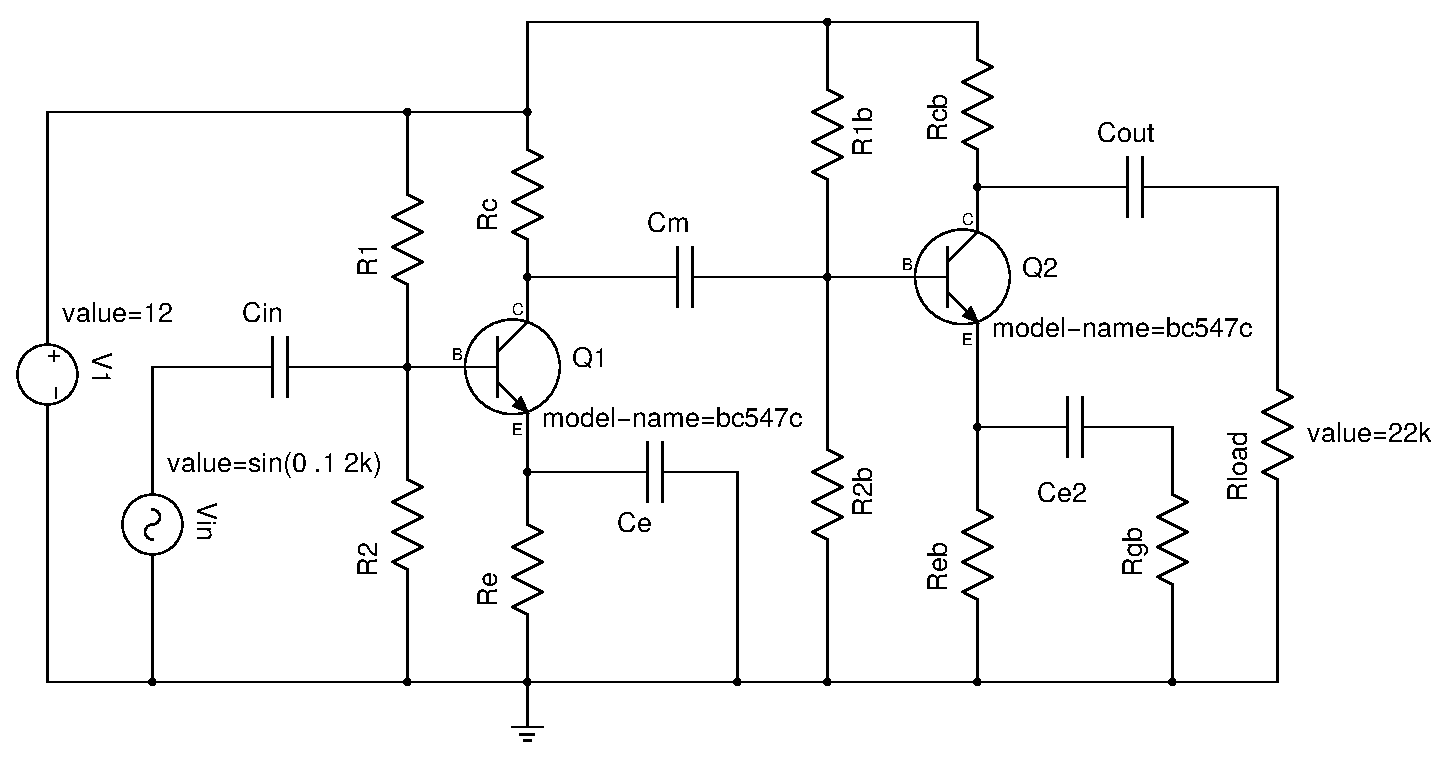
\includegraphics[scale=0.65]{ce-amplifier-2stage} \label{ce-amplifier-2stage}
    \caption{Circuit diagram for the two stage common emitter amplifier}
\end{figure}

\section{ngSPICE}
ngSPICE \footnote{ngSPICE home page - \url{http://ngspice.sourceforge.net/}} is an open-source, general-purpose circuit simulation program based on SPICE (\textit{Simulation Program with Integrated Circuit Emphasis}). It can simulate circuits with linear components and also nonlinear circuits which contain common semiconductor devices. Besides the simulation of analog circuits, it also offers simulation of digital circuits, in which case the simulator operates only with the logic states of the circuit, which has a great influence on the speed of the simulator. ngSPICE also offers a mixed-mode simulation where both the digital and analog simulations are combined together \cite{ngSPICE-manual}.

ngSPICE uses a language which syntax has been inherited from SPICE for describing circuits. An example of such description of the circuit from figure \ref{ce-amplifier} is shown in listing \ref{ce-amp-lst}. The first line contains the name of the circuit and on the next four lines, there is a description of the transistor used in the circuit. On the next lines, there is a list of the circuit's components. The name of the component is on the first position followed by the numbers or names of the nodes which the component is connected to. The last position contains the properties of the component. The second last line contains the description of the simulation. In this case, we do a transient analysis of the circuit for \SI{1.22}{\milli\second} with the sampling period \SI{20}{\micro\second} which provides the time course of the amplifier's output signal. Later on, we use this data to evaluate the amplifier's quality.

Such netlist can be generated by using the gEDA \footnote{gEDA home page - \url{http://geda-project.org/}} (\textit{Electronic Design Automation}) toolkit which is also an open-source project oriented towards electronic design.

\begin{lstlisting}[caption={description of the common emitter amplifier using the SPICE syntax},
    label={ce-amp-lst},
    captionpos=b,
    numbers=left]
 amplifier
.model bc547c NPN (BF=730 NE=1.4 ISE=29.5F IKF=80M IS=60F
       + VAF=25 ikr=12m BR=10 NC=2 VAR=10 RB=280 RE=1 RC=40
       + VJE=.48 tr=.3u tf=.5n cje=12p vje=.48 mje=.5
       + cjc=6p vjc=.7 mjc=.33 isc=47.6p kf=2f)
Vin in 0 sin(0 .1 2k)
V1 4 0 9
Ce 0 5 5u
Cout 1 out 220n
Cin in 3 220n
Rc 1 4 1k
Rload 0 out 22k
Re 0 5 1k
Rg 5 2 40
R2 0 3 33k
R1 3 4 47k
Q1 1 3 2 bc547c
.TRAN 20u 1.22m
.end
\end{lstlisting}

In figure \ref{ce-amplifier-sim} we can see the simulation output of the circuit from listing \ref{ce-amp-lst} which is the same circuit as in figure \ref{ce-amplifier}. This circuit was also built using real electronic components in order to verify the simulation results. The measurement results of the real circuit proved that the simulator works correctly for this circuit as the measured values corresponded to the simulation.

\begin{figure}[!ht]
    \centering
    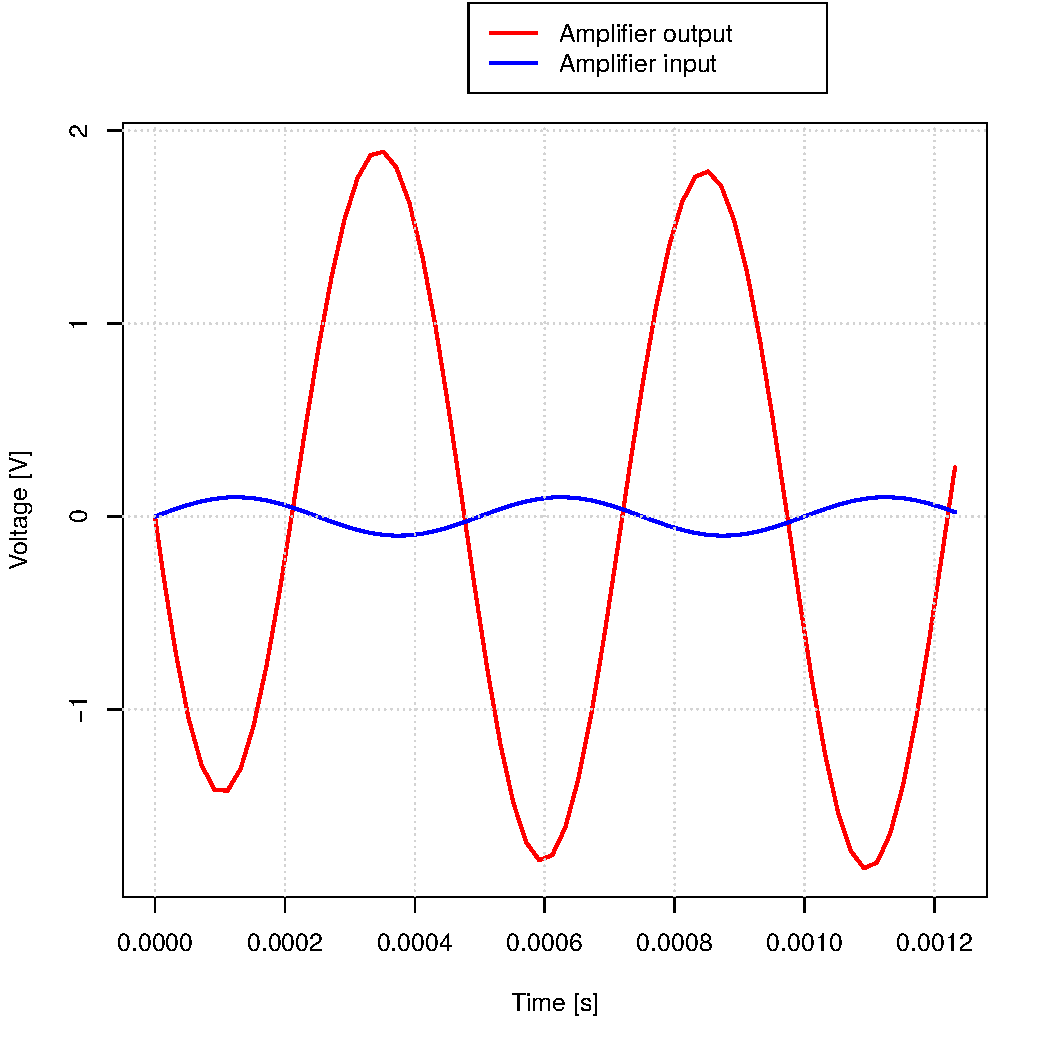
\includegraphics[scale=.6]{ce-amplifier-sim}\label{ce-amplifier-sim}
    \caption{Simulation of the single stage common emitter amplifier}
\end{figure}

The last version of ngSPICE offers a C API which makes the simulator the ideal choice for utilizing it with the evolutionary algorithms. Every chromosome (candidate solution) in the evolution represents one amplifier and the simulator is used to determine the quality of it.

The API is used to pass the description of the amplifier to the simulator, run the simulation and obtain the simulation results. The results are in the form of arrays in C which represent time and the corresponding voltage values. These arrays have an equal length which depends on the simulation duration and the sampling period.

The default input frequency for the amplifier is \SI{2}{\kilo\hertz}, the duration of the simulation is set to \SI{1.22}{\milli\second} and it contains approximately two and a half period of the output signal. The duration does not need to be longer because the shape of the waveform does not change after the cicuit gets to a stable state. The sampling period is \SI{20}{\micro\second} so that the waveform is smooth enough on one hand and the simulation does not take too long on the other hand. The array containing the output voltage is used for the evaluation of the chromosomes which is thoroughly discussed in chapter \ref{chromosomes-evaluation}.

The simulator is launched several thousand times during a typical evolution and it takes most of the computation time. During the implementation of the algorithms discussed in section \ref{evolution-strategies} and the integration of the simulator, it emerged that there are memory leaks on several places in the source code of the simulator. This was a problem as the simulator leaked memory in every iteration. A significant amount of time was spent on fixing these bugs and the result is that the memory leaks have been removed. These improvements were proposed as a patch to the development team and they will be incorporated into the next versions of ngSPICE.